\documentclass{article}

\usepackage{booktabs}
\usepackage{microtype}
\usepackage{pgfplots}
\title{Mandatory Assignment 1}
\author{Kris-Mikael Krister (krismikk)\\\texttt{krismikael@protonmail.com}}
\date{\today}

\begin{document}

\maketitle

\noindent This report describes five different methods for optimizing route distance for a set of cities, also known as the travelling salesman problem. The five methods are:

\begin{enumerate}
    \item Exhaustive search
    \item Hill climber
    \item Genetic algorithm
    \item Hybrid of 2) and 3) using a Lamarckian learning model
    \item Hybrid of 2) and 3) using a Baldwinian learning model
\end{enumerate}

\noindent Each method has an implemented algorithm written in Python. Python 3.4 or above is required to run some of the algorithms due to usage of the statistics library for standard deviation.

\section*{Exhaustive Search}

This algorithm is guaranteed to find the shortest path since all possible permutations are evaluated. From the set of the following ten cities, the path found to be shortest is Copenhagen $\rightarrow$ Hamburg $\rightarrow$ Brussels $\rightarrow$ Dublin $\rightarrow$ Barcelona $\rightarrow$ Belgrade $\rightarrow$ Istanbul $\rightarrow$ Bucharest $\rightarrow$ Budapest $\rightarrow$ Berlin. The total distance for the route is $7\,486.31$ km, and the solution was found using $21.25$ seconds\footnote{The computer used to run all implemented algorithms is a Linux i5-4670 CPU @ 3.40GHz.}. A single core was used when running the program, so exploiting the multi-core architecture would be a possible improvement to the program.  \\

\begin{center}
\begin{tabular}{crr}
\toprule
Number of cities & Permutations & Execution time (seconds)\\
\midrule
$5$ & $120$ & $0.00035$ \\
$6$ & $720$ & $0.0044$ \\
$7$ & $5\,040$ & $0.020$ \\
$8$ & $40\,320$ & $0.22$ \\
$9$ & $362\,880$ & $1.88$ \\
$10$ & $3\,628\,800$ & $21.25$ \\
$11$ & $39\,916\,800$ & $258$ \\
$12$ & $479\,001\,600$ & $3406.87$ \\
\bottomrule
\end{tabular}
\end{center}

\noindent Difference in execution time is proportional to the number of permutations. The amount of permutations is factorial ($O(n!)$), so based on the results above, the expected running time for all 24 cities would be approximately $3406.87 * 13 * 14 * \ldots * 24 \approx 4.41 \times 10^{18}$ seconds ($141\,962\,633\,400$ years).

\subsection*{How to run the program}

Execute the \texttt{tsp\_exhaustive.py} file with the amount of cities to check. Grab a coffee if you choose 12 or more cities.

\begin{verbatim}
$ python tsp_exhaustive.py 5

Exhastive search using 5 first cities
Found shortest {'distance': 4983.38, 'route': ('Barcelona',
'Belgrade', 'Bucharest', 'Berlin', 'Brussels')} in
0.00048303604126 seconds
\end{verbatim}

\section*{Hill Climber}

This section describes the results using a hill climber implementation to find the shortest path. In contrast to the exhaustive search, this algorithm is not guaranteed to find the global optima but will run significantly faster as we will see.

\subsection*{Implementation}

Key properties for the implementation are shown below.

\begin{itemize}
    \item A random permutation (route) is chosen as a starting point for the algorithm.
    \item The total distance for the route is calculated.
    \item The position of two random cities in the route are swapped, and the route distance is re-calculated.
    \item If the new route distance is shorter than the previous one, update the pointer of the best route.
    \item Repeat until the maximum amount of total iterations are reached (set to $5000$), or maximum amount of iterations (set to $50$) with a change below a threshold (set to $300$ km) is reached.
\end{itemize}

\subsection*{Results}

Each result may be different due to the stochastic nature of the algorithm. Twenty executions were used to get the numbers listed below.

\begin{center}
\begin{tabular}{lcc}
\toprule
Measurement & Ten cities & All cities \\
\midrule
Best & $7\,486.31$ km & $12\,759.8$ km \\
Worst & $8\,407.18$ & $15\,209.07$ \\
Mean & $7\,747.34$ & $14\,005.63$ \\
Standard deviation & $346.35$ & $821.67$ \\
Execution time & $0.94$ s & $2.09$ s \\
\bottomrule
\end{tabular}
\end{center}

\noindent Since the global optima was found in the exhaustive search, the results show that the hill climber found the shortest route for the case of the ten cities. The optimal solution for all cities is unknown.

\subsection*{How to run the program}

Execute the \texttt{tsp\_hill\_climber.py} file with the amount of cities to check.

\begin{verbatim}
$ python tsp_hill_climber.py 24

Hill climber search using first 24 cities. Running in total 20
iterations.
Best   12759.8
Worst  15209.069999999998
Mean   14005.635999999999
stdev  821.6690607307211
\end{verbatim}

\section*{Genetic Algorithm}

This section describes the results using a genetic algorithm to find the shortest path. The travelling salesman problem is a permutation problem, so the crossover and mutation operators must be chosen accordingly. The phenotype space is the set of city names. The crossover algorithm used is a partial mapped crossover algorithm. The algorithm is written to support array of city names as input so the genotype space can be the same as the phenotype.

\subsection*{Implementation}

The genetic algorithm runs three rounds with population size set to 50 the first round, 100 for the second and 200 for the third. Number of executions in each round is set to 20, and the best of these executions wins the round. Each execution iterates 100 generations to improve the population. A subset of the offspring is selected to form each of the following generations.

As with the previous tasks, all individuals in the population are routes, e.g. Berlin $\rightarrow$ Barcelona $\rightarrow$ $\ldots$ $\rightarrow$ Belgrade. Each individual has the same number of cities (genes). The general steps for the implementation are shown below.

\begin{enumerate}
    \item An initial population is randomly generated.
    \item The fitness for each individual is calculated. The fitness is based on the total route distance for the individual, compared to the total route distance for the entire population. The shortest route will have the highest fitness.
    \item The number of parents is set to half the population size, and parents are chosen using a stochastic universal sampling (SUS) method to avoid selection bias.
    \item Offspring is created using a partial mapped crossover algorithm. The number of offspring is set to double the amount of the population.
    \item The mutation strategy is \textit{swap two genes} up to two times per child. The initial mutation strategy was swap up to one time with probability $50\%$, but had to be adjusted as the population in that case in almost all cases converged towards having the same fitness. Mutation probablity $60\%$ plus a second round of swap with probability $40\%$ eliminated this symptom in all cases I tested.
    \item A $\mu,\lambda$ selection is used to form the next generation. All parents are discarded, and half of the $2 \times \lambda$ offspring are selected for the next generation. Individuals are prioritized by their fitness level.
\end{enumerate}

\subsection*{Results}

The results shows the best of the 20 executions for the three different population sizes.

\subsubsection*{Population size 50}

\begin{center}
\begin{tabular}{lcc}
\toprule
Measurement & Ten cities & All cities \\
\midrule
Best & $7\,486.31$ km & $12\,976.68$ km \\
Worst & $7\,503.10$ & $17\,288.78$ \\
Mean & $7\,488.82$ & $14\,086.72$ \\
Standard deviation & $6.15$ & $990.21$ \\
Execution time & $3.64$ s & $7.99$ s \\
\bottomrule
\end{tabular}
\end{center}

\subsubsection*{Population size 100}

\begin{center}
\begin{tabular}{lcc}
\toprule
Measurement & Ten cities & All cities \\
\midrule
Best & $7\,486.31$ km & $12\,287.07$ km \\
Worst & $7\,503.10$ & $15\,964.22$ \\
Mean & $7\,487.99$ & $13\,794.15$ \\
Standard deviation & $5.17$ & $1\,032.31$ \\
Execution time & $7.44$ s & $16.18$ s \\
\bottomrule
\end{tabular}
\end{center}

\subsubsection*{Population size 200}

\begin{center}
\begin{tabular}{lcc}
\toprule
Measurement & Ten cities & All cities \\
\midrule
Best & $7\,486.31$ km & $12\,771.46$ km \\
Worst & $7\,486.31$ & $14\,567.73$ \\
Mean & $7\,486.31$ & $13\,581.41$ \\
Standard deviation & $\approx 0$ & $396.53$ \\
Execution time & $15.33$ s & $33.12$ s \\
\bottomrule
\end{tabular}
\end{center}

% arstr.replace(/\s+/g, ' ').trim().split(' ').map((elem, index) => `(${index},${elem})`).join('')

\subsubsection*{Average values}

The following graph shows each generation's best value in average of the three population sizes (10 cities).

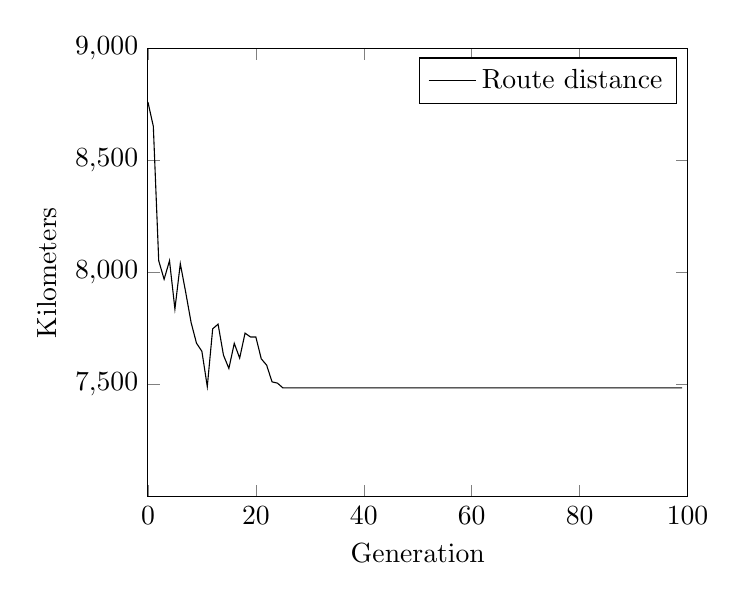
\begin{tikzpicture}
\begin{axis}[
    xlabel={Generation},
    ylabel={Kilometers},
    xmin=0, xmax=100,
    ymin=7000, ymax=9000,
    xtick={0,20,40,60,80,100},
    ytick={7500,8000,8500,9000}
]
\addplot[
]
coordinates {
    (0,8761.17333333)(1,8653.04666667)(2,8053.13333333)(3,7970.54333333)(4,8053.19666667)(5,7837.73333333)(6,8040.15)(7,7912.34333333)(8,7777.68666667)(9,7685.17666667)(10,7649.14333333)(11,7491.90666667)(12,7749.42666667)(13,7770.31333333)(14,7631.87333333)(15,7572.80666667)(16,7684.61)(17,7618.90333333)(18,7730.25333333)(19,7713.13666667)(20,7713.13666667)(21,7615.7)(22,7587.34)(23,7512.85666667)(24,7507.26)(25,7486.31)(26,7486.31)(27,7486.31)(28,7486.31)(29,7486.31)(30,7486.31)(31,7486.31)(32,7486.31)(33,7486.31)(34,7486.31)(35,7486.31)(36,7486.31)(37,7486.31)(38,7486.31)(39,7486.31)(40,7486.31)(41,7486.31)(42,7486.31)(43,7486.31)(44,7486.31)(45,7486.31)(46,7486.31)(47,7486.31)(48,7486.31)(49,7486.31)(50,7486.31)(51,7486.31)(52,7486.31)(53,7486.31)(54,7486.31)(55,7486.31)(56,7486.31)(57,7486.31)(58,7486.31)(59,7486.31)(60,7486.31)(61,7486.31)(62,7486.31)(63,7486.31)(64,7486.31)(65,7486.31)(66,7486.31)(67,7486.31)(68,7486.31)(69,7486.31)(70,7486.31)(71,7486.31)(72,7486.31)(73,7486.31)(74,7486.31)(75,7486.31)(76,7486.31)(77,7486.31)(78,7486.31)(79,7486.31)(80,7486.31)(81,7486.31)(82,7486.31)(83,7486.31)(84,7486.31)(85,7486.31)(86,7486.31)(87,7486.31)(88,7486.31)(89,7486.31)(90,7486.31)(91,7486.31)(92,7486.31)(93,7486.31)(94,7486.31)(95,7486.31)(96,7486.31)(97,7486.31)(98,7486.31)(99,7486.31)
};
\legend{Route distance}
\end{axis}
\end{tikzpicture}

\noindent The following graph shows each generation's best value in average of the three population sizes (24 cities).

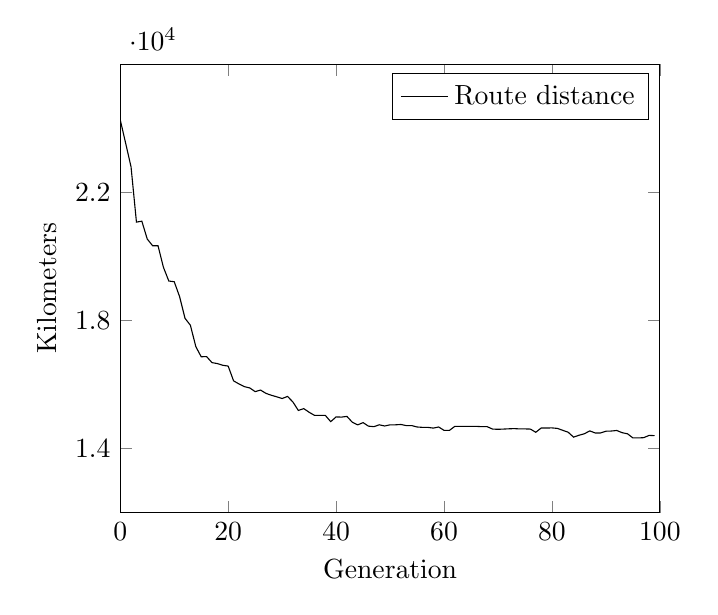
\begin{tikzpicture}
\begin{axis}[
    xlabel={Generation},
    ylabel={Kilometers},
    xmin=0, xmax=100,
    ymin=12000, ymax=26000,
    xtick={0,20,40,60,80,100},
    ytick={14000,18000,22000}
]
\addplot[
]
coordinates {
    (0,24262.53666667)(1,23532.69666667)(2,22792.76)(3,21068.52666667)(4,21097.56)(5,20541.21666667)(6,20329.74666667)(7,20329.74666667)(8,19657.55666667)(9,19228.71333333)(10,19207.2)(11,18739.79333333)(12,18064.93)(13,17847.37333333)(14,17180.91666667)(15,16864.02)(16,16869.42333333)(17,16680.98)(18,16650.8)(19,16598.36333333)(20,16572.02333333)(21,16111.1)(22,16015.06)(23,15930.62666667)(24,15890.63)(25,15774.97666667)(26,15823.85666667)(27,15720.61)(28,15661.66)(29,15612.65666667)(30,15560.02)(31,15624.99333333)(32,15450.73)(33,15187.18333333)(34,15245.30666667)(35,15130.53666667)(36,15033.34666667)(37,15033.34666667)(38,15033.34666667)(39,14837.58333333)(40,14985.53666667)(41,14979.47)(42,15002.23666667)(43,14818.79666667)(44,14737.81333333)(45,14807.00666667)(46,14696.78)(47,14681.09666667)(48,14739.08)(49,14701.81666667)(50,14739.08)(51,14739.08)(52,14749.15)(53,14715.01)(54,14715.01)(55,14671.05333333)(56,14659.17)(57,14659.17)(58,14635.78666667)(59,14671.05333333)(60,14565.74333333)(61,14565.74333333)(62,14690.33333333)(63,14690.33333333)(64,14690.33333333)(65,14690.33333333)(66,14690.33333333)(67,14680.16666667)(68,14680.16666667)(69,14605.61666667)(70,14598.81)(71,14605.61666667)(72,14614.16)(73,14620.15333333)(74,14611.04)(75,14611.04)(76,14605.61666667)(77,14505.73)(78,14638.82666667)(79,14638.82666667)(80,14642.46)(81,14626.95666667)(82,14566.81666667)(83,14507.73333333)(84,14353.58333333)(85,14412.59)(86,14459.44666667)(87,14549.70666667)(88,14484.55333333)(89,14484.55333333)(90,14539.06)(91,14544.45333333)(92,14562.16666667)(93,14493.5)(94,14457.81)(95,14329.78666667)(96,14329.78666667)(97,14337.27)(98,14408.49)(99,14401.00666667)
};
\legend{Route distance}
\end{axis}
\end{tikzpicture}

\subsubsection*{All three population sizes}

The following graph shows each generation's best value for each of the population sizes (10 cities).

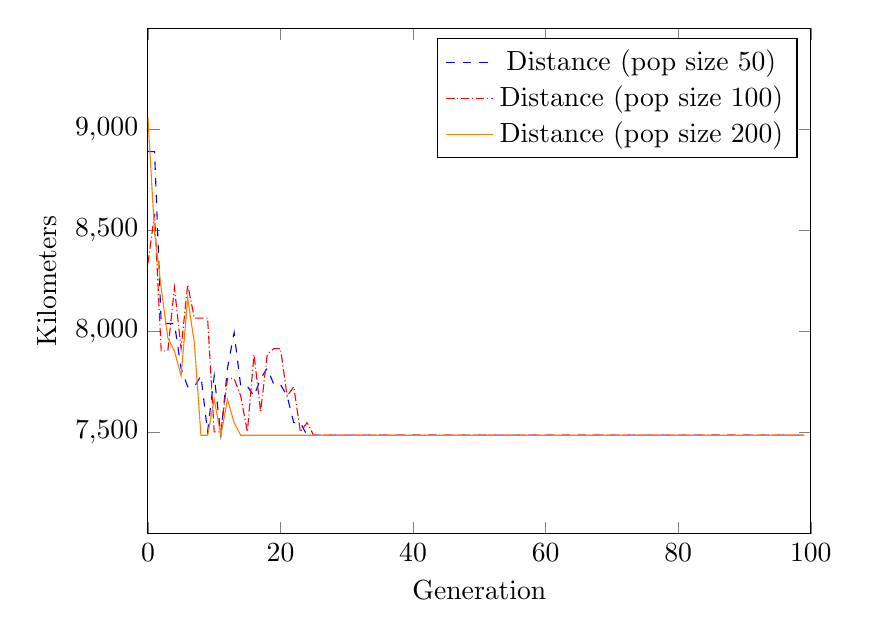
\begin{tikzpicture}
\begin{axis}[
    xlabel={Generation},
    ylabel={Kilometers},
    width=10cm, height=8cm,
    xmin=0, xmax=100,
    ymin=7000, ymax=9500,
    xtick={0,20,40,60,80,100},
    ytick={7500,8000,8500,9000}
]
\addplot[
color=blue,
dashed
]
coordinates {
    (0,8890.090000000002)(1,8889.52)(2,8039.19)(3,8039.19)(4,8039.19)(5,7817.42)(6,7726.36)(7,7726.36)(8,7780.63)(9,7503.1)(10,7780.63)(11,7486.31)(12,7817.42)(13,7994.62)(14,7729.009999999999)(15,7729.009999999999)(16,7680.490000000001)(17,7767.16)(18,7817.42)(19,7737.950000000001)(20,7737.950000000001)(21,7680.490000000001)(22,7549.16)(23,7549.16)(24,7486.3099999999995)(25,7486.3099999999995)(26,7486.3099999999995)(27,7486.3099999999995)(28,7486.3099999999995)(29,7486.3099999999995)(30,7486.3099999999995)(31,7486.3099999999995)(32,7486.3099999999995)(33,7486.3099999999995)(34,7486.3099999999995)(35,7486.3099999999995)(36,7486.3099999999995)(37,7486.3099999999995)(38,7486.3099999999995)(39,7486.3099999999995)(40,7486.3099999999995)(41,7486.3099999999995)(42,7486.3099999999995)(43,7486.3099999999995)(44,7486.3099999999995)(45,7486.3099999999995)(46,7486.3099999999995)(47,7486.3099999999995)(48,7486.3099999999995)(49,7486.3099999999995)(50,7486.3099999999995)(51,7486.3099999999995)(52,7486.3099999999995)(53,7486.3099999999995)(54,7486.3099999999995)(55,7486.3099999999995)(56,7486.3099999999995)(57,7486.3099999999995)(58,7486.3099999999995)(59,7486.3099999999995)(60,7486.3099999999995)(61,7486.3099999999995)(62,7486.3099999999995)(63,7486.3099999999995)(64,7486.3099999999995)(65,7486.3099999999995)(66,7486.3099999999995)(67,7486.3099999999995)(68,7486.3099999999995)(69,7486.3099999999995)(70,7486.3099999999995)(71,7486.3099999999995)(72,7486.3099999999995)(73,7486.3099999999995)(74,7486.3099999999995)(75,7486.3099999999995)(76,7486.3099999999995)(77,7486.3099999999995)(78,7486.3099999999995)(79,7486.3099999999995)(80,7486.3099999999995)(81,7486.3099999999995)(82,7486.3099999999995)(83,7486.3099999999995)(84,7486.3099999999995)(85,7486.3099999999995)(86,7486.3099999999995)(87,7486.3099999999995)(88,7486.3099999999995)(89,7486.3099999999995)(90,7486.3099999999995)(91,7486.3099999999995)(92,7486.3099999999995)(93,7486.3099999999995)(94,7486.3099999999995)(95,7486.3099999999995)(96,7486.3099999999995)(97,7486.3099999999995)(98,7486.3099999999995)(99,7486.3099999999995)
};
\addlegendentry{Distance (pop size 50)}
\addplot[
color=red,
densely dashdotted
]
coordinates {
    (0,8336.03)(1,8582.1)(2,7903.82)(3,7903.82)(4,8216.58)(5,7915.339999999999)(6,8232.17)(7,8066.12)(8,8066.12)(9,8066.12)(10,7503.1)(11,7503.1)(12,7767.16)(13,7767.16)(14,7680.299999999999)(15,7503.1)(16,7887.03)(17,7603.24)(18,7887.03)(19,7915.150000000001)(20,7915.150000000001)(21,7680.299999999999)(22,7726.550000000001)(23,7503.1)(24,7549.16)(25,7486.310000000001)(26,7486.310000000001)(27,7486.310000000001)(28,7486.310000000001)(29,7486.310000000001)(30,7486.310000000001)(31,7486.310000000001)(32,7486.310000000001)(33,7486.310000000001)(34,7486.310000000001)(35,7486.310000000001)(36,7486.310000000001)(37,7486.310000000001)(38,7486.310000000001)(39,7486.310000000001)(40,7486.310000000001)(41,7486.310000000001)(42,7486.310000000001)(43,7486.310000000001)(44,7486.310000000001)(45,7486.310000000001)(46,7486.310000000001)(47,7486.310000000001)(48,7486.310000000001)(49,7486.310000000001)(50,7486.310000000001)(51,7486.310000000001)(52,7486.310000000001)(53,7486.310000000001)(54,7486.310000000001)(55,7486.310000000001)(56,7486.310000000001)(57,7486.310000000001)(58,7486.310000000001)(59,7486.310000000001)(60,7486.310000000001)(61,7486.310000000001)(62,7486.310000000001)(63,7486.310000000001)(64,7486.310000000001)(65,7486.310000000001)(66,7486.310000000001)(67,7486.310000000001)(68,7486.310000000001)(69,7486.310000000001)(70,7486.310000000001)(71,7486.310000000001)(72,7486.310000000001)(73,7486.310000000001)(74,7486.310000000001)(75,7486.310000000001)(76,7486.310000000001)(77,7486.310000000001)(78,7486.310000000001)(79,7486.310000000001)(80,7486.310000000001)(81,7486.310000000001)(82,7486.310000000001)(83,7486.310000000001)(84,7486.310000000001)(85,7486.310000000001)(86,7486.310000000001)(87,7486.310000000001)(88,7486.310000000001)(89,7486.310000000001)(90,7486.310000000001)(91,7486.310000000001)(92,7486.310000000001)(93,7486.310000000001)(94,7486.310000000001)(95,7486.310000000001)(96,7486.310000000001)(97,7486.310000000001)(98,7486.310000000001)(99,7486.310000000001)
};
\addlegendentry{Distance (pop size 100)}
\addplot[
color=orange,
]
coordinates {
    (0,9057.4)(1,8487.519999999999)(2,8216.390000000001)(3,7968.619999999999)(4,7903.820000000001)(5,7780.44)(6,8161.92)(7,7944.55)(8,7486.3099999999995)(9,7486.3099999999995)(10,7663.7)(11,7486.3099999999995)(12,7663.7)(13,7549.16)(14,7486.3099999999995)(15,7486.3099999999995)(16,7486.3099999999995)(17,7486.3099999999995)(18,7486.3099999999995)(19,7486.3099999999995)(20,7486.3099999999995)(21,7486.3099999999995)(22,7486.3099999999995)(23,7486.3099999999995)(24,7486.3099999999995)(25,7486.3099999999995)(26,7486.3099999999995)(27,7486.3099999999995)(28,7486.3099999999995)(29,7486.3099999999995)(30,7486.3099999999995)(31,7486.3099999999995)(32,7486.3099999999995)(33,7486.3099999999995)(34,7486.3099999999995)(35,7486.3099999999995)(36,7486.3099999999995)(37,7486.3099999999995)(38,7486.3099999999995)(39,7486.3099999999995)(40,7486.3099999999995)(41,7486.3099999999995)(42,7486.3099999999995)(43,7486.3099999999995)(44,7486.3099999999995)(45,7486.3099999999995)(46,7486.3099999999995)(47,7486.3099999999995)(48,7486.3099999999995)(49,7486.3099999999995)(50,7486.3099999999995)(51,7486.3099999999995)(52,7486.3099999999995)(53,7486.3099999999995)(54,7486.3099999999995)(55,7486.3099999999995)(56,7486.3099999999995)(57,7486.3099999999995)(58,7486.3099999999995)(59,7486.3099999999995)(60,7486.3099999999995)(61,7486.3099999999995)(62,7486.3099999999995)(63,7486.3099999999995)(64,7486.3099999999995)(65,7486.3099999999995)(66,7486.3099999999995)(67,7486.3099999999995)(68,7486.3099999999995)(69,7486.3099999999995)(70,7486.3099999999995)(71,7486.3099999999995)(72,7486.3099999999995)(73,7486.3099999999995)(74,7486.3099999999995)(75,7486.3099999999995)(76,7486.3099999999995)(77,7486.3099999999995)(78,7486.3099999999995)(79,7486.3099999999995)(80,7486.3099999999995)(81,7486.3099999999995)(82,7486.3099999999995)(83,7486.3099999999995)(84,7486.3099999999995)(85,7486.3099999999995)(86,7486.3099999999995)(87,7486.3099999999995)(88,7486.3099999999995)(89,7486.3099999999995)(90,7486.3099999999995)(91,7486.3099999999995)(92,7486.3099999999995)(93,7486.3099999999995)(94,7486.3099999999995)(95,7486.3099999999995)(96,7486.3099999999995)(97,7486.3099999999995)(98,7486.3099999999995)(99,7486.3099999999995)
};
\addlegendentry{Distance (pop size 200)}
\end{axis}
\end{tikzpicture}

The following graph shows each generation's best value for each of the population sizes (all cities).

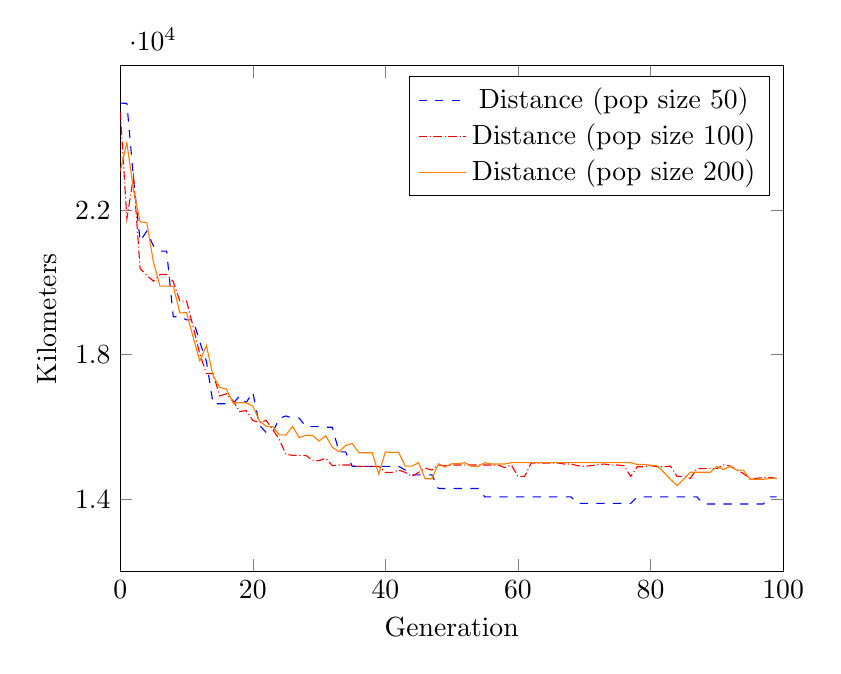
\begin{tikzpicture}
\begin{axis}[
    xlabel={Generation},
    ylabel={Kilometers},
    xmin=0, xmax=100,
    ymin=12000, ymax=26000,
    xtick={0,20,40,60,80,100},
    width=10cm, height=8cm,
    ytick={14000,18000,22000}
]
\addplot[
color=blue,
dashed
]
coordinates {
    (0,24969.59)(1,24962.659999999996)(2,22875.34)(3,21144.85)(4,21423.31000000001)(5,21014.899999999998)(6,20867.690000000002)(7,20867.690000000002)(8,19051.100000000006)(9,19051.100000000006)(10,18965.770000000004)(11,18965.770000000004)(12,18348.340000000004)(13,17816.880000000005)(14,16642.350000000002)(15,16642.350000000002)(16,16642.350000000002)(17,16642.350000000002)(18,16857.290000000005)(19,16674.450000000004)(20,16962.280000000002)(21,16047.140000000003)(22,15848.730000000003)(23,15848.730000000003)(24,16243.280000000002)(25,16303.74)(26,16243.280000000002)(27,16243.280000000002)(28,16006.380000000001)(29,16006.380000000001)(30,16006.380000000001)(31,15990.270000000002)(32,15990.270000000002)(33,15306.86)(34,15306.86)(35,14907.51)(36,14907.51)(37,14907.51)(38,14907.51)(39,14907.51)(40,14907.51)(41,14907.51)(42,14907.51)(43,14805.380000000003)(44,14672.86)(45,14672.86)(46,14672.86)(47,14672.86)(48,14294.740000000002)(49,14294.740000000002)(50,14294.740000000002)(51,14294.740000000002)(52,14294.740000000002)(53,14294.740000000002)(54,14294.740000000002)(55,14060.45)(56,14060.45)(57,14060.45)(58,14060.45)(59,14060.45)(60,14060.45)(61,14060.45)(62,14060.45)(63,14060.45)(64,14060.45)(65,14060.45)(66,14060.45)(67,14060.45)(68,14060.45)(69,13880.41)(70,13880.41)(71,13880.41)(72,13880.41)(73,13880.41)(74,13880.41)(75,13880.41)(76,13880.41)(77,13880.41)(78,14060.45)(79,14060.45)(80,14060.45)(81,14060.45)(82,14060.45)(83,14060.45)(84,14060.45)(85,14060.45)(86,14060.45)(87,14060.45)(88,13864.989999999998)(89,13864.989999999998)(90,13864.989999999998)(91,13864.989999999998)(92,13864.989999999998)(93,13864.989999999998)(94,13864.989999999998)(95,13864.989999999998)(96,13864.989999999998)(97,13864.989999999998)(98,14060.45)(99,14060.45)
};
\addlegendentry{Distance (pop size 50)}
\addplot[
color=red,
densely dashdotted
]
coordinates {
    (0,24735.03)(1,21768.109999999993)(2,22937.209999999995)(3,20380.390000000003)(4,20207.89)(5,20035.300000000003)(6,20220.4)(7,20220.4)(8,20020.420000000002)(9,19477.94)(10,19490.33)(11,18772.030000000002)(12,18018.14)(13,17474.98)(14,17474.98)(15,16857.879999999997)(16,16917.519999999997)(17,16730.91)(18,16425.64)(19,16450.960000000003)(20,16181.06)(21,16113.929999999998)(22,16181.06)(23,15927.759999999998)(24,15650.050000000001)(25,15242.63)(26,15212.9)(27,15212.9)(28,15212.9)(29,15065.89)(30,15065.89)(31,15133.050000000001)(32,14925.16)(33,14943.72)(34,14943.72)(35,14943.72)(36,14907.029999999999)(37,14907.029999999999)(38,14907.029999999999)(39,14907.029999999999)(40,14739.169999999998)(41,14739.169999999998)(42,14807.470000000001)(43,14739.169999999998)(44,14628.74)(45,14739.169999999998)(46,14854.52)(47,14807.470000000001)(48,14943.72)(49,14922.58)(50,14943.72)(51,14943.72)(52,14943.72)(53,14943.72)(54,14943.72)(55,14943.72)(56,14943.72)(57,14943.72)(58,14873.570000000002)(59,14943.72)(60,14627.790000000003)(61,14627.790000000003)(62,15001.56)(63,15001.56)(64,15001.56)(65,15001.56)(66,15001.56)(67,14971.060000000001)(68,14971.060000000001)(69,14927.45)(70,14907.029999999999)(71,14927.45)(72,14953.079999999998)(73,14971.060000000001)(74,14943.72)(75,14943.72)(76,14927.45)(77,14627.790000000003)(78,14896.950000000003)(79,14896.950000000003)(80,14927.45)(81,14896.950000000003)(82,14896.950000000003)(83,14913.220000000001)(84,14627.790000000003)(85,14627.790000000003)(86,14574.84)(87,14845.62)(88,14845.62)(89,14845.62)(90,14845.62)(91,14948.61)(92,14916.240000000002)(93,14813.95)(94,14706.880000000001)(95,14574.84)(96,14574.84)(97,14597.290000000005)(98,14597.290000000005)(99,14574.84)
};
\addlegendentry{Distance (pop size 100)}
\addplot[
color=orange,
]
coordinates {
    (0,23082.989999999998)(1,23867.320000000003)(2,22565.729999999996)(3,21680.340000000004)(4,21661.48)(5,20573.450000000004)(6,19901.15)(7,19901.15)(8,19901.15)(9,19157.099999999995)(10,19165.499999999996)(11,18481.58)(12,17828.31)(13,18250.260000000002)(14,17425.420000000002)(15,17091.83)(16,17048.4)(17,16669.68)(18,16669.47)(19,16669.68)(20,16572.73)(21,16172.230000000001)(22,16015.39)(23,16015.39)(24,15778.560000000001)(25,15778.560000000001)(26,16015.39)(27,15705.650000000001)(28,15765.7)(29,15765.7)(30,15607.789999999999)(31,15751.66)(32,15436.76)(33,15310.97)(34,15485.34)(35,15540.380000000001)(36,15285.5)(37,15285.5)(38,15285.5)(39,14698.21)(40,15309.93)(41,15291.73)(42,15291.73)(43,14911.84)(44,14911.84)(45,15008.989999999998)(46,14562.959999999997)(47,14562.959999999997)(48,14978.779999999999)(49,14888.130000000001)(50,14978.779999999999)(51,14978.779999999999)(52,15008.989999999998)(53,14906.57)(54,14906.57)(55,15008.989999999998)(56,14973.34)(57,14973.34)(58,14973.34)(59,15008.989999999998)(60,15008.989999999998)(61,15008.989999999998)(62,15008.989999999998)(63,15008.989999999998)(64,15008.989999999998)(65,15008.989999999998)(66,15008.989999999998)(67,15008.989999999998)(68,15008.989999999998)(69,15008.989999999998)(70,15008.989999999998)(71,15008.989999999998)(72,15008.989999999998)(73,15008.989999999998)(74,15008.989999999998)(75,15008.989999999998)(76,15008.989999999998)(77,15008.989999999998)(78,14959.079999999998)(79,14959.079999999998)(80,14939.48)(81,14923.470000000001)(82,14743.05)(83,14549.529999999999)(84,14372.509999999998)(85,14549.529999999999)(86,14743.05)(87,14743.05)(88,14743.05)(89,14743.05)(90,14906.57)(91,14819.760000000002)(92,14905.27)(93,14801.560000000001)(94,14801.560000000001)(95,14549.529999999999)(96,14549.529999999999)(97,14549.529999999999)(98,14567.73)(99,14567.73)
};
\addlegendentry{Distance (pop size 200)}
\end{axis}
\end{tikzpicture}

\subsection*{Conclusion}

Based on the results shown above, the different population sizes chosen doesn't affect the result noticably. The improvement per generation is approximately the same for all three population sizes, and the improvement rate converges at around 25 generations for 10 cities, and 50-60 generations for 24 cities. In this example, the lowest population size of 50 performed best in regards to finding the shortest route \textit{and} execution time. Although the difference is low, it's noticable when including all cities. However, due to the stochastic nature of the algorithm and the low difference in results, I cannot conclude that the population size of 50 will be the best in all runs.

\subsubsection*{Execution time}

For the case of 10 cities, the shortest route was found for all three population sizes. For the 24 cities, the shortest route found was $12\,287$ km. In regards to execution time, the GA is slower than the Hill Climber algorithm, but faster than the exhaustive search for all tested population sizes. The following table displays the results.

\begin{center}
\begin{tabular}{lcc}
\toprule
Algorithm & Ten cities & All cities \\
\midrule
Hill climber & $0.94$ s & $2.09$ s \\
Exhaustive search & $21.25$ & $4.41 \times 10^{18}$ (estimated) \\
Genetic (population 50) & $3.64$ & $7.99$ \\
Genetic (population 100) & $7.44$ & $16.18$ \\
Genetic (population 200) & $15.33$ & $33.12$ \\
\bottomrule
\end{tabular}
\end{center}

\subsubsection*{Tours inspected}

All permutations ($O(n!)$) are inspected in the exhaustive search. The GA inspects the population size $\lambda$ for each of the generations times the executions. Note that the number of inspected routes for the GA is not correlated with the number of cities. When $\lambda = 50$, number of generations $= 100$ with $20$ executions the number of inspected routes are as follows.

\begin{center}
\begin{tabular}{lcc}
\toprule
Algorithm & Ten cities & All cities \\
\midrule
Exhaustive search & $3\,628\,800$ & $620\,448\,401\,733\,239\,439\,360\,000$ \\
Genetic (population 50) & $100\,000$ & $100\,000$ \\
\bottomrule
\end{tabular}
\end{center}

\subsection*{How to run the program}

Execute the \texttt{tsp\_genetic.py} file with the amount of cities to check.

\begin{verbatim}
$ python tsp_genetic.py 24
\end{verbatim}

\section*{Hybrid Algorithm}

This section describes the result when combining hill climbing with the genetic algorithm. The hill climber improves (or tries to improve) each individual before selecting survivors for next generation. Otherwise, run the genetic algorithm as described in the previous section. There are two variants to this strategy, \textbf{the Lamarckian} and the \textbf{the Baldwinian}, and they differ in how the hill climber results are used for the genotype of the upcoming generation.

\subsection*{Results using the Lamarckian learning model}

The results from the hill climber are \textit{kept in the genotype} in the Lamarckian learning model. The results below shows the best of the 20 executions for the three different population sizes.

\subsubsection*{Population size 50}

\begin{center}
\begin{tabular}{lcc}
\toprule
Measurement & Ten cities & All cities \\
\midrule
Best & $7\,486.31$ km & $12\,287.07$ km \\
Worst & $7\,486.31$ & $14\,551.74$ \\
Mean & $7\,486.31$ & $13\,148.74$ \\
Standard deviation & $\approx 0$ & $627.53$ \\
Execution time & $23.45$ s & $53.78$ s \\
\bottomrule
\end{tabular}
\end{center}

\subsubsection*{Population size 100}

\begin{center}
\begin{tabular}{lcc}
\toprule
Measurement & Ten cities & All cities \\
\midrule
Best & $7\,486.31$ km & $12\,325.93$ km \\
Worst & $7\,486.31$ & $13\,947.42$ \\
Mean & $7\,486.31$ & $12\,921.10$ \\
Standard deviation & $\approx 0$ & $473.40$ \\
Execution time & $47.17$ s & $107.66$ s \\
\bottomrule
\end{tabular}
\end{center}

\subsubsection*{Population size 200}

\begin{center}
\begin{tabular}{lcc}
\toprule
Measurement & Ten cities & All cities \\
\midrule
Best & $7\,486.31$ km & $12\,287.07$ km \\
Worst & $7\,486.31$ & $13\,459.37$ \\
Mean & $7\,486.31$ & $12\,676.69$ \\
Standard deviation & $\approx 0$ & $285.59$ \\
Execution time & $94.57$ s & $215.95$ s \\
\bottomrule
\end{tabular}
\end{center}

\subsubsection*{Average values}

The following graph shows each generation's best value in average of the three population sizes (10 cities). Note that the x axis is smaller than the previous graphs since the data converged towards the optima very fast.

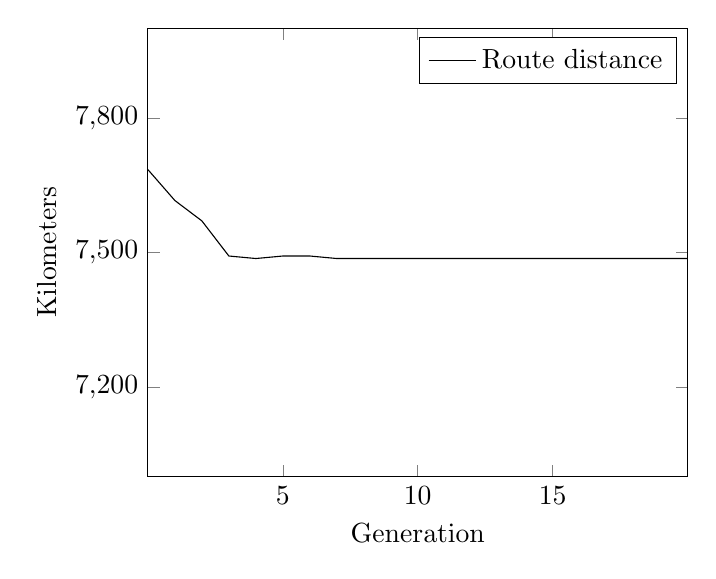
\begin{tikzpicture}
\begin{axis}[
    xlabel={Generation},
    ylabel={Kilometers},
    xmin=0, xmax=20,
    ymin=7000, ymax=8000,
    xtick={5,10,15},
    ytick={7200,7500,7800}
]
\addplot[
]
coordinates {
    (0,7684.61)(1,7615.63666667)(2,7570.19)(3,7491.90666667)(4,7486.31)(5,7491.90666667)(6,7491.90666667)(7,7486.31)(8,7486.31)(9,7486.31)(10,7486.31)(11,7486.31)(12,7486.31)(13,7486.31)(14,7486.31)(15,7486.31)(16,7486.31)(17,7486.31)(18,7486.31)(19,7486.31)(20,7486.31)(21,7486.31)(22,7486.31)(23,7486.31)(24,7486.31)(25,7486.31)(26,7486.31)(27,7486.31)(28,7486.31)(29,7486.31)(30,7486.31)(31,7486.31)(32,7486.31)(33,7486.31)(34,7486.31)(35,7486.31)(36,7486.31)(37,7486.31)(38,7486.31)(39,7486.31)(40,7486.31)(41,7486.31)(42,7486.31)(43,7486.31)(44,7486.31)(45,7486.31)(46,7486.31)(47,7486.31)(48,7486.31)(49,7486.31)(50,7486.31)(51,7486.31)(52,7486.31)(53,7486.31)(54,7486.31)(55,7486.31)(56,7486.31)(57,7486.31)(58,7486.31)(59,7486.31)(60,7486.31)(61,7486.31)(62,7486.31)(63,7486.31)(64,7486.31)(65,7486.31)(66,7486.31)(67,7486.31)(68,7486.31)(69,7486.31)(70,7486.31)(71,7486.31)(72,7486.31)(73,7486.31)(74,7486.31)(75,7486.31)(76,7486.31)(77,7486.31)(78,7486.31)(79,7486.31)(80,7486.31)(81,7486.31)(82,7486.31)(83,7486.31)(84,7486.31)(85,7486.31)(86,7486.31)(87,7486.31)(88,7486.31)(89,7486.31)(90,7486.31)(91,7486.31)(92,7486.31)(93,7486.31)(94,7486.31)(95,7486.31)(96,7486.31)(97,7486.31)(98,7486.31)(99,7486.31)
};
\legend{Route distance}
\end{axis}
\end{tikzpicture}

\noindent The following graph shows each generation's best value in average of the three population sizes (24 cities).

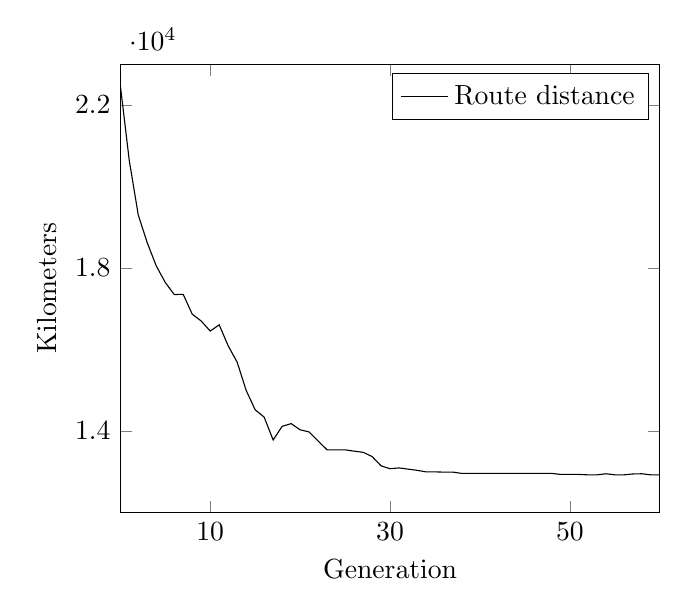
\begin{tikzpicture}
\begin{axis}[
    xlabel={Generation},
    ylabel={Kilometers},
    xmin=0, xmax=60,
    ymin=12000, ymax=23000,
    xtick={10,30,50},
    ytick={14000,18000,22000}
]
\addplot[
]
coordinates {
    (0,22496.75)(1,20639.99666667)(2,19302.67)(3,18618.73666667)(4,18052.36)(5,17645.97333333)(6,17348.57333333)(7,17353.28)(8,16868.12666667)(9,16698.06333333)(10,16452.5)(11,16604.91333333)(12,16090.81666667)(13,15687.20666667)(14,14995.4)(15,14520.47333333)(16,14340.90333333)(17,13779.42)(18,14114.7)(19,14181.08333333)(20,14028.95)(21,13977.67666667)(22,13753.46)(23,13537.96)(24,13537.96)(25,13537.96)(26,13505.77333333)(27,13477.26666667)(28,13374.02666667)(29,13144.66333333)(30,13074.44)(31,13094.74)(32,13064.37)(33,13035.44)(34,12996.99)(35,12996.99)(36,12990.92333333)(37,12990.92333333)(38,12958.99)(39,12958.99)(40,12958.99)(41,12958.99)(42,12958.99)(43,12958.99)(44,12958.99)(45,12958.99)(46,12958.99)(47,12958.99)(48,12958.99)(49,12934.18666667)(50,12934.18666667)(51,12934.18666667)(52,12924.27)(53,12924.27)(54,12950.94)(55,12924.27)(56,12924.27)(57,12945.95666667)(58,12950.94)(59,12924.27)(60,12924.27)(61,12924.27)(62,12924.27)(63,12924.27)(64,12924.27)(65,12924.27)(66,12924.27)(67,12958.99)(68,12958.99)(69,12924.27)(70,12924.27)(71,12910.04333333)(72,12924.27)(73,12912.89666667)(74,12912.89666667)(75,12912.89666667)(76,12912.89666667)(77,12912.89666667)(78,12845.1)(79,12924.27)(80,12919.96)(81,12919.96)(82,12934.18666667)(83,12958.99)(84,12890.43)(85,12890.43)(86,12915.23333333)(87,12879.82)(88,12879.82)(89,12879.82)(90,12879.82)(91,12873.44666667)(92,12855.01666667)(93,12855.01666667)(94,12855.01666667)(95,12879.82)(96,12879.82)(97,12879.82)(98,12879.82)(99,12879.82)
};
\legend{Route distance}
\end{axis}
\end{tikzpicture}


\subsection*{Results using the Baldwinian learning model}

The difference from the Baldwinian model compared to the Lamarckian is that improvements from the hill climber are only used to \textit{prioritize the population}, and no changes are made to the genotype. The results below show the best of the 20 executions for the three different population sizes.

\subsubsection*{Population size 50}

\begin{center}
\begin{tabular}{lcc}
\toprule
Measurement & Ten cities & All cities \\
\midrule
Best & $7\,486.31$ km & $13\,670.69$ km \\
Worst & $7\,663.51$ & $15\,599.32$ \\
Mean & $7\,516.82$ & $14\,462.36$ \\
Standard deviation & $54.85$ & $659.37$ \\
Execution time & $23.39$ s & $53.71$ s \\
\bottomrule
\end{tabular}
\end{center}

\subsubsection*{Population size 100}

\begin{center}
\begin{tabular}{lcc}
\toprule
Measurement & Ten cities & All cities \\
\midrule
Best & $7\,486.31$ km & $12\,744.34$ km \\
Worst & $7\,680.49$ & $15\,415.12$ \\
Mean & $7\,500.84$ & $13\,993.13$ \\
Standard deviation & $44.72$ & $750.64$ \\
Execution time & $47.01$ s & $108.26$ s \\
\bottomrule
\end{tabular}
\end{center}

\subsubsection*{Population size 200}

\begin{center}
\begin{tabular}{lcc}
\toprule
Measurement & Ten cities & All cities \\
\midrule
Best & $7\,486.31$ km & $12\,679.14$ km \\
Worst & $7\,737.95$ & $14\,794.53$ \\
Mean & $7\,521.14$ & $13\,835.83$ \\
Standard deviation & $78.49$ & $573.73$ \\
Execution time & $95.04$ s & $218.01$ s \\
\bottomrule
\end{tabular}
\end{center}

\subsubsection*{Average values}

The following graph shows each generation's best value in average of the three population sizes (10 cities).

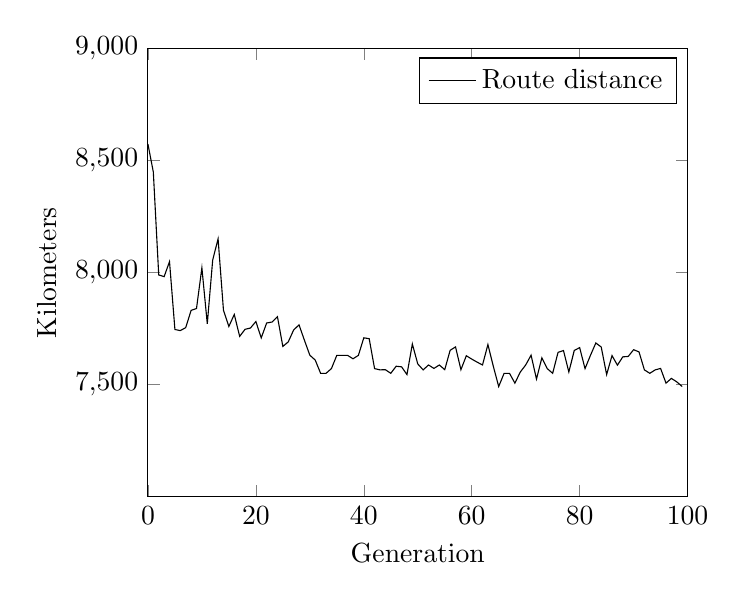
\begin{tikzpicture}
\begin{axis}[
    xlabel={Generation},
    ylabel={Kilometers},
    xmin=0, xmax=100,
    ymin=7000, ymax=9000,
    xtick={0,20,40,60,80,100},
    ytick={7500,8000,8500,9000}
]
\addplot[
]
coordinates {
    (0,8573.74)(1,8448.90333333)(2,7989.92666667)(3,7982.16666667)(4,8049.21333333)(5,7746.50333333)(6,7741.48666667)(7,7754.73666667)(8,7831.64)(9,7840.16)(10,8021.6)(11,7771.73333333)(12,8056.32666667)(13,8150.92333333)(14,7831.63333333)(15,7760.07)(16,7813.59333333)(17,7715.75333333)(18,7747.39)(19,7752.98666667)(20,7781.94)(21,7709.27333333)(22,7775.48)(23,7779.78333333)(24,7803.58666667)(25,7670.91333333)(26,7691.00333333)(27,7744.35)(28,7767.11333333)(29,7698.54)(30,7631.87333333)(31,7610.10333333)(32,7551.03666667)(33,7550.97333333)(34,7571.98666667)(35,7631.11666667)(36,7631.11666667)(37,7631.11666667)(38,7615.76333333)(39,7631.05333333)(40,7709.27333333)(41,7705.56)(42,7571.98666667)(43,7566.39)(44,7567.21)(45,7551.03666667)(46,7582.57333333)(47,7579.92666667)(48,7545.44)(49,7681.78666667)(50,7592.93666667)(51,7566.32666667)(52,7588.16)(53,7572.80666667)(54,7588.16)(55,7567.21)(56,7653.48333333)(57,7668.85)(58,7567.21)(59,7629.32)(60,7614.50666667)(61,7600.87666667)(62,7588.16)(63,7679.23333333)(64,7582.57333333)(65,7491.90666667)(66,7551.03666667)(67,7551.03666667)(68,7507.26)(69,7556.63333333)(70,7588.17)(71,7631.93666667)(72,7525.28666667)(73,7620.10333333)(74,7571.98666667)(75,7551.03666667)(76,7644.65333333)(77,7652.67666667)(78,7556.63333333)(79,7652.89666667)(80,7665.60333333)(81,7571.92333333)(82,7630.99)(83,7686.21333333)(84,7668.18666667)(85,7545.44)(86,7630.06)(87,7587.34)(88,7624.47333333)(89,7626.25333333)(90,7656.40666667)(91,7646.43)(92,7566.32666667)(93,7550.97333333)(94,7566.32666667)(95,7572.80666667)(96,7507.26)(97,7528.21)(98,7512.85666667)(99,7491.90666667)
};
\legend{Route distance}
\end{axis}
\end{tikzpicture}

\noindent The following graph shows each generation's best value in average of the three population sizes (24 cities).

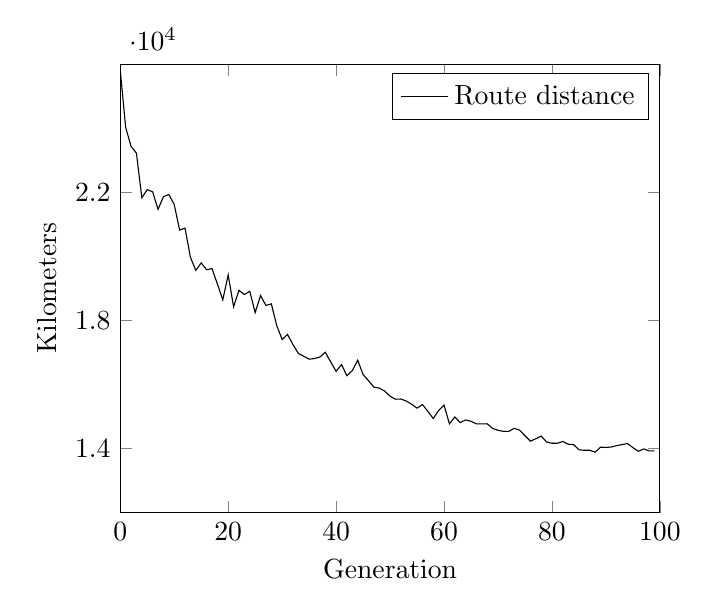
\begin{tikzpicture}
\begin{axis}[
    xlabel={Generation},
    ylabel={Kilometers},
    xmin=0, xmax=100,
    ymin=12000, ymax=26000,
    xtick={0,20,40,60,80,100},
    ytick={14000,18000,22000}
]
\addplot[
]
coordinates {
    (0,25815.38333333)(1,24028.17)(2,23436.20666667)(3,23220.38333333)(4,21830.04666667)(5,22081.40333333)(6,22015.86)(7,21469.11)(8,21861.51333333)(9,21932.15333333)(10,21616.46)(11,20819.58333333)(12,20882.74)(13,19970.04333333)(14,19560.92666667)(15,19795.54666667)(16,19582.13)(17,19615.22333333)(18,19137.85333333)(19,18639.92333333)(20,19420.48666667)(21,18423.24)(22,18940.43)(23,18806.57333333)(24,18909.59)(25,18242.23333333)(26,18775.51333333)(27,18466.64333333)(28,18515.43)(29,17834.96)(30,17402.35)(31,17560.04333333)(32,17247.07333333)(33,16969.15333333)(34,16879.94333333)(35,16787.8)(36,16809.87333333)(37,16855.99333333)(38,17003.99666667)(39,16701.4)(40,16409.12666667)(41,16620.26)(42,16271.34)(43,16431.08)(44,16757.41333333)(45,16306.73)(46,16116.14)(47,15915.15333333)(48,15885.87666667)(49,15791.81666667)(50,15631.53666667)(51,15538.06)(52,15544.64)(53,15480.73666667)(54,15379.40666667)(55,15260.02666667)(56,15371.68333333)(57,15159.82333333)(58,14934.05666667)(59,15187.34666667)(60,15355.09666667)(61,14770.87666667)(62,14984.50333333)(63,14807.7)(64,14890.93)(65,14848.00333333)(66,14767.81333333)(67,14767.81333333)(68,14770.75666667)(69,14627.99)(70,14568.86)(71,14534.67666667)(72,14534.67666667)(73,14628.70333333)(74,14570.41333333)(75,14397.08333333)(76,14229.43)(77,14303.06)(78,14386.98666667)(79,14203.57)(80,14162.19)(81,14162.19)(82,14218.41333333)(83,14133.31666667)(84,14121.20333333)(85,13958.51666667)(86,13942.89666667)(87,13942.89666667)(88,13883.76666667)(89,14040.20333333)(90,14032.32)(91,14046.73333333)(92,14089.86)(93,14120.96666667)(94,14154.37666667)(95,14026.83)(96,13911.66666667)(97,13985.70333333)(98,13923.58)(99,13923.58)
};
\legend{Route distance}
\end{axis}
\end{tikzpicture}

\subsection*{Conclusion}

A swift convergence towards an optima is seen when using the Lamarckian learning model. The results for these executions show that the hybrid model performs at least equal to the pure genetic algorithm to find the shortest route distance, but finds it faster. It may be they both found the global optima of $12,287.07$ km (not confirmed). It's also possible that the shortest route found is a \textit{local} optima, and the Lamarckian just got stuck there faster than the pure genetic one. Both hybrid models are slower to run than the pure genetic algorithm by a factor of $6-7$, and they are also more complex to write. Since the results indicate the algorithm converge quickly, the number of generations can be reduced to improve the execution time.

The Baldwinian learning model performs worst in regard to finding the route distance. However, as shown in the graphs above, the Baldwinian model is better at a continuous exploration of the genotype space.

\end{document}
